% PLOS ONE submission
% Initial submission format: article class, single-column
% https://journals.plos.org/plosone/s/submission-guidelines

\documentclass[11pt,a4paper]{article}

% === Packages ===
\usepackage[margin=2.5cm]{geometry}
\usepackage[numbers,sort&compress]{natbib}
\usepackage{graphicx}
\usepackage{booktabs}
\usepackage{amsmath,amssymb}
\usepackage{hyperref}
\usepackage{setspace}
\usepackage{enumitem}
\onehalfspacing
\setlength{\parskip}{4pt}
\setlength{\emergencystretch}{2em}

\begin{document}

% ===== TITLE PAGE =====
\title{\LARGE\bfseries From Noisy Conflict Scores to Forecastable Risk States in Social Media Comment Streams}

\author{
Linli Zhu\\[2pt]
{\small School of Computer Science, Ningxia University, Yinchuan, China}\\[2pt]
{\small violina2333@gmail.com}\\[6pt]
Ziqiang Ma$^\ast$\\[2pt]
{\small School of Information Engineering, Ningxia University, Yinchuan, China}\\[2pt]
{\small maziqiang@nxu.edu.cn}\\[6pt]
$^\ast$ Corresponding author
}
\date{}

\maketitle

% ===== ABSTRACT =====
\noindent\textbf{Abstract}

Social media conflict forecasting promises earlier intervention than post-hoc content classification, yet raw text-derived scores are sparse and temporally noisy. We construct a conflict index without task-specific labels and introduce a leakage-resistant cleaning pipeline that regularizes the 12-hour time axis, learns all calibration and cleaning statistics from training data only, and performs causal exponential smoothing. A logistic model predicts whether the stabilized state will exceed the topic-specific training-period 80th percentile within the next six bins. Smoothing, regularization, decision threshold, and feature-set complexity are selected on validation data; the final 25\% of each topic is held out for testing. The validation rule selects a parsimonious state-history model. Across 20 Zhihu topics and 1,706 test windows, it achieves AUC $0.891$, precision $0.738$, recall $0.822$, and F1 $0.778$, compared with persistence recall $0.584$ and F1 $0.716$. Topic-level paired bootstrap confirms gains in F1 ($+0.062$, 95\% CI $[0.018,0.108]$) and recall ($+0.241$, $[0.173,0.317]$); F1 improves on 15 of 20 topics. Results remain positive at 70th, 80th, and 90th-percentile risk definitions. Continuous-value regression remains below persistence, showing that causal state modeling supports high-risk-state prediction but not exact trajectory forecasting.

\noindent\textbf{Keywords:} conflict index, risk-state prediction, social media comments, temporal validation, causal smoothing, public opinion monitoring

\newpage

% ═══════════════════════════════════════════════
\section{Introduction}
% ═══════════════════════════════════════════════

\subsection{Challenges in Governing Social Media Public Opinion}

The ubiquity of social media has transformed how information is produced, circulated, and contested. Public debates that once unfolded over days now escalate within hours as platforms enable rapid information cascades and viral diffusion~\cite{Vosoughi2018}. Seemingly marginal topics can ignite large-scale opinion swings with tangible offline consequences. For example, coordinated online discourse has been shown to correlate with mass protests and even violent incidents in subsequent days~\cite{Steinert2015,Arcila2024}. 

\textbf{Information Cascades and Offline Spillovers.} Information spreads faster than it can be verified. Emotional contagion and algorithmic amplification jointly fuel cascades that can spill over into offline actions. Once critical mass is reached, moderation or fact-checking becomes less effective, as narratives solidify through repeated exposure~\cite{Vosoughi2018}. These cascades thus demand proactive, not reactive, management.

\textbf{Delays in Post-hoc Sentiment Analysis.} Conventional sentiment analysis frameworks primarily offer retrospective insight: they describe how people felt after events unfolded. However, by the time significant polarity shifts are detected, the discussion may already have escalated beyond control. This latency between event occurrence and analytical response undermines the capacity for early intervention~\cite{Wang2020}.

\textbf{Research Gaps in Proactive Monitoring.} Despite advances in opinion mining and social listening, few studies explicitly target anticipatory modeling. Existing tools classify emotions or toxicity per message, but rarely attempt to forecast when online discontent is likely to escalate~\cite{Wang2020}. This absence of anticipatory modeling creates a crucial gap between detection and prevention.

\subsection{Limitations of Existing Technical Paradigms}

\textbf{Lexicon/Rule-Based Systems.} Lexicon-based or rule-driven systems offer interpretability but struggle with context-dependent semantics, sarcasm, and multilingual variation. Irony (``Great, another perfect policy!'') or cultural idioms can easily invert meaning~\cite{Dhumpati2025}. Moreover, such systems require language-specific dictionaries that fail in cross-lingual or code-mixed environments~\cite{Kaity2020}.

\textbf{Static Classifiers.} Traditional supervised classifiers are trained on fixed datasets and assume distributional stability. In dynamic online environments, vocabulary, sentiment norms, and social topics evolve rapidly---an issue known as concept drift~\cite{Gama2014}. Without continuous adaptation, static models degrade, misclassify emergent patterns, or fail to generalize to unseen contexts.

\textbf{Post-Level Analysis without Temporal Modeling.} Recent pretrained language models substantially improve post-level semantic understanding, sentiment recognition, and harmful-content detection. However, these methods score or classify comments independently, without explicitly modeling how conflict accumulates and evolves across time. Consequently, they provide informative local signals but limited support for topic-level escalation forecasting. This motivates the introduction of a temporal forecasting layer on top of interpretable post-level risk signals~\cite{Abdalgader2025}.

\subsection{Contributions of This Work}

To address the above limitations, we construct the upstream conflict index without task-specific labels and evaluate supervised downstream predictors under leakage-resistant temporal protocols. The main contributions are:

\begin{enumerate}[leftmargin=*,itemsep=2pt]
\item \textbf{Conflict-index quantification framework.} An index constructed without task-specific labels combines attack-related intensity, negative high-arousal emotion, and stance polarization into a unified post-level score. We explicitly test rather than assume whether its aggregated trajectory is forecastable.

\item \textbf{Leakage-resistant state construction.} We restore the regular time grid and learn clipping, imputation, scaling, smoothing, risk thresholds, and classifier settings without accessing the final test period.

\item \textbf{Positive but bounded real-data result.} The selected state-history classifier improves F1 and recall over persistence on most Zhihu topics. Threshold and feature ablations show that the causal state, rather than additional noisy semantic components, drives the gain.

\item \textbf{Forecastability boundary.} Continuous regression remains persistence-dominated on real semantic trajectories, whereas synthetic trajectories and objective Weibo activity are predictable. This separates useful monitoring-state classification from unsupported claims of exact conflict forecasting.
\end{enumerate}

% ═══════════════════════════════════════════════
\section{Related Work}
% ═══════════════════════════════════════════════

\subsection{Deep Learning for Sentiment and Emotion Understanding}

Deep learning has significantly advanced sentiment analysis by learning contextual and compositional linguistic patterns. Transformer-based architectures, particularly BERT and its multilingual variants, have achieved strong results across diverse sentiment benchmarks by leveraging self-attention mechanisms that capture long-range dependencies~\cite{bert-multilingual-sentiment}. Pre-training on large corpora enables these models to capture nuanced affective signals, including intensity gradients, mixed emotions, and context-dependent polarity shifts. Recent domain-adaptive approaches and fine-tuning strategies have further improved robustness across platforms and languages~\cite{wahid2025crisis,birjali2021sentiment}.

\subsection{Risk Scoring for Harmful Content and Hazardous Conversations}

Beyond categorical sentiment labels, risk scoring aims to assign continuous severity estimates to online content. Toxicity classifiers assign continuous scores for hate speech, personal attacks, and harassment~\cite{Wulczyn2017}. These models provide per-comment severity levels but do not model how individual toxic comments cumulatively contribute to topic-level risk over time. Their temporal dimension---whether early toxic comments are predictive of later escalation---remains largely unexplored. Recent models for harmful meme detection and safe speech classification~\cite{ghosh2024safespeech} and stance detection~\cite{kucuk2020stance,paschalides2025polar} further enrich content-level signals but share the same temporal limitation.

\subsection{Temporal Forecasting of Public Opinion Trends with LSTM Variants}

LSTM-based architectures dominate time-series forecasting of public opinion dynamics. The IPSO-LSTM hybrid~\cite{Mu2023IPSO} uses particle swarm optimization for hyperparameter tuning. TRESP~\cite{Zhang2024TRESP} incorporates self-attention mechanisms to weight temporal influences. Informer~\cite{zhou2021informer} and its Lite variant address long-sequence efficiency. CNN-LSTM hybrids have been proposed for crisis prediction~\cite{lou2024cnnlstm,singh2025cupcdlstm,upadhyay2024satcobilstm}. The memory-cycle properties of time-series public opinion data have also been investigated~\cite{liu2025memory}. However, these works typically operate on aggregate time series or manual labels without integrating fine-grained, post-level semantic evidence in an unsupervised manner.

\subsection{Information Cascade and Diffusion Prediction}

A parallel line of work studies how content spreads through social networks. Predictive models of information cascades~\cite{xu2025d2,xu2025hyperidp} focus on diffusion depth and breadth rather than semantic conflict escalation. Separately, recent evidence from Weibo conflict discourse networks demonstrates that affective homophily---emotional similarity between users---rather than structural prestige, is the dominant organizing principle in online conflict~\cite{gu2025affective}. This validates the central role of negative high-arousal emotion in our conflict-index formulation. The echo-chamber amplification identified in~\cite{ghafouri2024echo} further corroborates the importance of stance polarization signals.

\subsection{Fundamental Problem: Evaluation Protocol}

A critical but often overlooked issue in this literature is the evaluation protocol. Standard cross-validation with random shuffling violates the temporal ordering of time-series data, artificially inflating performance metrics by allowing models to train on future observations~\cite{Bergmeir2012}. This practice is widespread in public-opinion forecasting papers but rarely acknowledged. Our work explicitly quantifies the magnitude of this inflation and advocates for temporal-split evaluation as a minimum standard.

% ═══════════════════════════════════════════════
\section{Methods}
% ═══════════════════════════════════════════════

\subsection{Problem Definition}

Let a comment stream from a social media topic be represented as a sequence of time bins $t = 1, 2, \dots, T$. Each bin $t$ contains $n_t$ comments $\{x_{t,1}, \dots, x_{t,n_t}\}$. First, we construct a conflict index $c_{t,i} \in [0,1]$ for each comment and aggregate it as $\bar{c}_t$. We then examine two downstream tasks: exact $H$-step trajectory regression and prediction of whether a stabilized, topic-relative high-risk state will occur within the next $H$ bins.

\subsection{Conflict-Index Quantification without Manual Labels}

For each comment $x_{t,i}$ in bin $t$, we compute three raw component scores.

\textbf{Attack/Antagonism Intensity.} Attack intensity $a_{t,i}$ is obtained from a pretrained multilingual BERT sentiment classifier~\cite{bert-multilingual-sentiment} (nlptown/bert-base-multilingual-uncased-sentiment) that outputs 5-class rating probabilities. The attack score is defined as:
\begin{equation}
a_{t,i} = p_{\text{1-star}} + 0.5 \cdot p_{\text{2-star}},
\label{eq:attack_score}
\end{equation}
where $p_{\text{1-star}}$ is the probability of the most negative rating class.

\textbf{Emotion Intensity.} We construct a composite emotion score that combines negative sentiment with an anger-like arousal component:
\begin{equation}
e_{t,i} = 0.7 \cdot (p_{\text{1-star}} + p_{\text{2-star}}) + 0.3 \cdot p_{\text{1-star}}.
\label{eq:emotion_score}
\end{equation}
This rewards comments that are both negative and emotionally intense, which are common precursors to conflict escalation.

\textbf{Stance Polarization via Within-Bin Semantic Bimodality.} Without stance labels, we estimate polarization from the semantic structure of comments within each time bin. Sentence embeddings $\mathbf{v}_{t,i} \in \mathbb{R}^{384}$ are obtained from a multilingual MiniLM-L12-v2 model~\cite{wang2020minilm}. Within each bin $t$, we cluster all embeddings into $k{=}2$ camps using K-Means. Let $\mathbf{u}_{t,1}, \mathbf{u}_{t,2}$ be the cluster centroids. The between-camp separation is:
\begin{equation}
\Delta_t = 1 - \cos(\mathbf{u}_{t,1}, \mathbf{u}_{t,2}).
\label{eq:camp_separation}
\end{equation}
Each comment's alignment confidence is:
\begin{equation}
q_{t,i} = \frac{|d(\mathbf{v}_{t,i}, \mathbf{u}_{t,1}) - d(\mathbf{v}_{t,i}, \mathbf{u}_{t,2})|}{d(\mathbf{v}_{t,i}, \mathbf{u}_{t,1}) + d(\mathbf{v}_{t,i}, \mathbf{u}_{t,2}) + \epsilon},
\label{eq:alignment_confidence}
\end{equation}
where $d(\cdot,\cdot)$ is cosine distance and $\epsilon = 10^{-8}$. For each topic, K-means is fitted only on embeddings before the exact 60\% regular-grid cutoff; its fixed centers then score validation and test comments. The stance score is:
\begin{equation}
s_{t,i} = \min(1, \Delta_t) \cdot q_{t,i}.
\label{eq:stance_score}
\end{equation}

\textbf{Distribution Calibration by Percentile Mapping.} We calibrate each raw score using empirical cumulative distribution function (ECDF) mapping. The calibrator (QuantileTransformer with $n_{\text{quantiles}}=1000$, uniform output) is fitted exclusively on the temporal training portion of each topic to prevent distributional leakage from the test set. This yields calibrated scores $\tilde{a}_{t,i}, \tilde{e}_{t,i}, \tilde{s}_{t,i}$.

\textbf{Comment-Level Fusion.} The calibrated scores are fused into a single conflict index:
\begin{equation}
c_{t,i} = \sigma\!\left(w_a \tilde{a}_{t,i} + w_e \tilde{e}_{t,i} + w_s \tilde{s}_{t,i} + b\right) \in [0,1],
\label{eq:conflict_index_fusion}
\end{equation}
where $\sigma$ is the sigmoid, and the default weights are $w_a:w_e:w_s = 0.5:0.3:0.2$.

\textbf{Bin-Level Aggregation.} Comment-level indices are aggregated into bin-level risk trajectories using top-$k$ mean aggregation. For each bin $t$, we retain the top $\lceil \rho n_t \rceil$ comments by conflict score and compute their mean, with $\rho = 0.15$:
\begin{equation}
\bar{c}_t = \frac{1}{\lceil \rho n_t \rceil} \sum_{j=1}^{\lceil \rho n_t \rceil} c_t^{(j)},
\label{eq:topk_agg}
\end{equation}
where $c_t^{(j)}$ are the sorted conflict scores in bin $t$. This emphasizes the high-risk tail of the comment distribution.

\subsection{CNN-BiLSTM Temporal Forecasting}

\textbf{Input Windowing and Forecast Target.} Given the bin-level trajectory $\bar{c}_t$, we construct sliding windows of length $L$ and forecast horizon $H$:
\begin{equation}
\mathbf{x}_t = [\bar{c}_{t-L+1}, \dots, \bar{c}_t]^\top \in \mathbb{R}^L,
\quad
\mathbf{y}_t = [\bar{c}_{t+1}, \dots, \bar{c}_{t+H}]^\top \in \mathbb{R}^H.
\label{eq:lstm_input_window}
\end{equation}
We set $L=12$ and $H=6$ in all experiments.

\textbf{Architecture.} The CNN-BiLSTM forecaster consists of: (i) a two-layer 1D convolutional front-end with 32 filters (kernel sizes 3 and 5, ReLU activation) to extract local temporal patterns; (ii) a two-layer bidirectional LSTM with 64 hidden units per direction and dropout 0.2 to model long-range dependencies; (iii) a linear projection head that maps the concatenated final hidden states to the $H$-step forecast.

\textbf{Training.} Training minimizes the Huber loss ($\delta=0.5$) using the Adam optimizer with learning rate $10^{-3}$ and a plateau-based scheduler. Early stopping with patience 25 is applied. All models are implemented in PyTorch and trained on a single NVIDIA GPU.

\textbf{Sequential Benchmark Inference.} At the end of each bin $t$, the CNN-BiLSTM maps the latest window to an $H$-step continuous forecast. We use this architecture as a benchmark; the real-data risk-state result below uses logistic regression.

\subsection{Leakage-Resistant Risk-State Prediction}

Retained Zhihu observations are first mapped back to the complete 12-hour grid because only 39.8\% of adjacent retained bins are truly consecutive. For each topic, the earliest 60\% of bins form training data, the next 15\% validation data, and the final 25\% the untouched test segment. Winsorization limits, imputation values, and scaling parameters are learned from training data only. Missing bins are imputed causally, and a missingness indicator is retained in the candidate feature pool.

We stabilize the cleaned index $z_t$ with a causal exponentially weighted moving average:
\begin{equation}
q_t=\alpha z_t+(1-\alpha)q_{t-1},\qquad \alpha=\frac{2}{S+1}.
\label{eq:ewma}
\end{equation}
Candidate spans $S\in\{12,18,24,30,36,48\}$ are compared using validation F1; $S=24$ is selected. Let $Q_{0.8}^{\mathrm{train}}$ be the topic-specific 80th percentile of $q_t$ in training. The prospective label is
\begin{equation}
y_t=\mathbb{1}\!\left[\max_{1\le h\le H}q_{t+h}>Q_{0.8}^{\mathrm{train}}\right].
\label{eq:risk_label}
\end{equation}
Windows require at least two observed future bins. We evaluate four nested feature groups: state only; state plus activity and missingness; state plus semantic components; and the full pool. For logistic regression, $C\in\{0.01,0.03,0.1,0.3,1.0\}$ and probability cutoffs from 0.30 to 0.70 are selected on validation F1. We choose the smallest feature group within 0.005 F1 of the best validation result. This selects the preceding $L=12$ states, $C=0.3$, and cutoff 0.30. No test observations influence preprocessing or model selection.

\subsection{Datasets}

\textbf{Real-World Zhihu Dataset.} The dataset contains approximately 45K comments and answers from 140 controversial topics on Zhihu, a Chinese Q\&A platform. After conflict-index construction and requiring at least three records in an observed 12-hour bin, 20 topics contain sufficient temporal coverage for risk-state analysis. Regularization and window construction yield 1,428 training, 680 validation, and 1,706 test windows.

\textbf{Synthetic Conflict Trajectories.} To enable controlled quantitative evaluation with known escalation labels, we generate 60 synthetic conflict trajectories of 200 bins each. Each trajectory is the sum of four components:
\begin{equation}
y_t = \beta + \tau_t + s_t + \varepsilon_t,
\label{eq:synthetic}
\end{equation}
where $\beta \sim \mathcal{U}(0.3, 0.45)$ is a topic-dependent baseline, $\tau_t$ comprises 1--3 logistic escalation events (sigmoid rise with exponential decay, amplitude 0.15--0.35, width 5--15 bins), $s_t$ is a weekly sinusoidal seasonality term ($\sigma=0.02$), and $\varepsilon_t$ is pink noise (AR(1), $\phi=0.6$, $\sigma_{\text{white}}=0.02$). Escalation events are labeled as ground truth when the trend contribution $\tau_t > 0.1$. The resulting trajectories exhibit realistic properties: mean conflict values in $[0.3, 0.7]$, event-driven volatility, and a 17.2\% prevalence of escalation bins.

\textbf{Weibo Reversal Events.} The Weibo Public Opinion Reversal Dataset~\cite{Zhang2023Reversal} contains 27 Chinese social-media controversy events (245K comments total) with manually annotated reversal time windows. Comment density is high (60--97 comments per hour during active events), enabling analysis of whether data sparsity alone explains the conflict index's failure on Zhihu.

\subsection{Baselines}

Twelve models are compared across three categories:

\textit{Statistical models:} Persistence ($\hat{c}_{t+h} = \bar{c}_t$), Moving Average with $k{=}3$, Exponential Smoothing with $\alpha{=}0.3$, and AR(6) fitted via ordinary least squares.

\textit{Classical machine learning:} Support Vector Regression with RBF kernel ($C{=}1.0$, $\gamma{=}\text{scale}$) and XGBoost (100 trees, max depth 6).

\textit{Deep architectures:} TCN (4-layer dilated convolution), Informer-Lite (prob-sparse attention), BiLSTM, Transformer with learnable positional encoding, BiGRU, and our CNN-BiLSTM.

\subsection{Evaluation Metrics and Protocol}

\textbf{Metrics.} We report R\textsuperscript{2}, Mean Absolute Error (MAE), and Root Mean Squared Error (RMSE) for regression. Risk-state prediction is evaluated by area under the ROC curve (AUC), precision, recall, and F1. Synthetic escalation uses the generator's trend contribution $>0.1$.

\textbf{Temporal-Split Protocol.} All experiments preserve temporal ordering and never shuffle windows. Synthetic benchmarks use 75\% training and 25\% testing. The real risk-state experiment uses 60\% training, 15\% validation, and 25\% testing per topic. ECDF calibration and every preprocessing or selection step are fitted without the test period. Deep models are evaluated over five independent seeds (42, 59, 76, 93, 110). Topic-level paired bootstrap with 10,000 resamples quantifies classifier differences from persistence.

% ═══════════════════════════════════════════════
\section{Results}
% ═══════════════════════════════════════════════

\subsection{Research Questions}

Our experiments address five research questions. \textbf{RQ1:} What temporal artifacts and noise limit the raw conflict index? \textbf{RQ2:} Can training-only cleaning and causal state histories improve held-out high-risk-state prediction over persistence? \textbf{RQ3:} How well do sequence models recover deliberately embedded continuous dynamics? \textbf{RQ4:} How sensitive are conclusions to signal components, features, risk thresholds, and noise? \textbf{RQ5:} What is the empirical lead time relative to synthetic escalation onset?

\subsection{Conflict-Index Trajectories on Real Data (RQ1)}

Table~\ref{tab:trajectory_stats} summarizes properties of the conflict-index trajectories computed from the five most active Zhihu topics. The conflict index shows topic-dependent mean levels (0.54--0.72) and standard deviations (0.03--0.04), indicating that the index captures meaningful between-topic variation. Cross-sectional validity is further supported by the Weibo case study (Sec.~\ref{sec:case_study}), where conflict-index shifts are observed during annotated reversal windows.

\begin{table}[ht]
\centering
\caption{Conflict-index trajectory statistics for the five most active Zhihu topics.}
\label{tab:trajectory_stats}
\begin{tabular}{lccc}
\toprule
\textbf{Topic} & \textbf{Bins} & \textbf{Conflict Index Range} & \textbf{Std} \\
\midrule
E-commerce refunds & 595 & [0.54, 0.72] & 0.024 \\
High-speed rail quiet cars & 589 & [0.51, 0.71] & 0.045 \\
Education in matchmaking & 506 & [0.52, 0.72] & 0.042 \\
Divorce cooling-off period & 454 & [0.56, 0.73] & 0.031 \\
Women in the workplace & 453 & [0.52, 0.72] & 0.033 \\
\bottomrule
\end{tabular}
\end{table}

\subsection{Synthetic Forecasting Performance (RQ2)}

Table~\ref{tab:forecast_results} reports full forecasting results under the strict temporal-split protocol ($\sim$8,235 training windows, $\sim$2,745 test windows). The deep sequential models---BiGRU (R\textsuperscript{2}=$0.811\pm0.009$), CNN-BiLSTM ($0.809\pm0.010$), and Transformer ($0.806\pm0.007$)---form a tight top tier with overlapping confidence intervals, all significantly outperforming non-neural baselines. The progression from statistical baselines through classical ML to deep architectures demonstrates consistent gains: XGBoost (R\textsuperscript{2}=$0.781$) improves substantially over AR(6) (R\textsuperscript{2}=$0.715$) through non-linear feature interactions, and the deep models further improve by 2--4 percentage points. BiGRU ($0.811$) and CNN-BiLSTM ($0.809$) are statistically indistinguishable ($\Delta$R\textsuperscript{2}=$-0.002$, within one standard deviation). The Transformer with learnable positional encoding achieves competitive results, demonstrating that self-attention architectures can match recurrent models on short sequences ($L{=}12$). Informer-Lite (R\textsuperscript{2}=$0.796$) shows no advantage over the standard Transformer at this sequence length.

\begin{table}[ht]
\centering
\caption{Forecasting results on synthetic trajectories (temporal split: 75\% train / 25\% test, $L{=}12$, $H{=}6$). Metrics are mean $\pm$ std over 5 independent seeds.}
\label{tab:forecast_results}
\begin{tabular}{lcccc}
\toprule
\textbf{Model} & \textbf{R\textsuperscript{2}} & \textbf{MAE} & \textbf{RMSE} & \textbf{Esc-F1} \\
\midrule
Persistence & 0.638$\pm$0.015 & 0.0317 & 0.0548 & 0.637 \\
Moving Avg (k=3) & 0.540$\pm$0.020 & 0.0370 & 0.0617 & 0.547 \\
Exp.\ Smoothing & 0.498$\pm$0.022 & 0.0379 & 0.0645 & 0.430 \\
AR(6) & 0.715$\pm$0.011 & 0.0293 & 0.0486 & 0.644 \\
SVR~\cite{Mu2023IPSO} & 0.759$\pm$0.024 & 0.0222 & 0.0448 & 0.667 \\
XGBoost & 0.781$\pm$0.013 & 0.0232 & 0.0427 & 0.684 \\
TCN & 0.787$\pm$0.010 & 0.0238 & 0.0421 & 0.695 \\
Informer-Lite & 0.796$\pm$0.014 & 0.0232 & 0.0413 & 0.659 \\
BiLSTM & 0.805$\pm$0.011 & 0.0227 & 0.0403 & 0.711 \\
Transformer + PE & 0.806$\pm$0.007 & 0.0227 & 0.0402 & 0.697 \\
BiGRU & 0.811$\pm$0.009 & 0.0221 & 0.0397 & \textbf{0.716} \\
CNN-BiLSTM & \textbf{0.809}$\pm$\textbf{0.010} & \textbf{0.0223} & \textbf{0.0398} & \textbf{0.710} \\
\bottomrule
\end{tabular}
\vspace{4pt}
{\small All results under strict temporal ordering with ECDF calibration on training data only.}
\end{table}

\begin{figure}[ht]
\centering
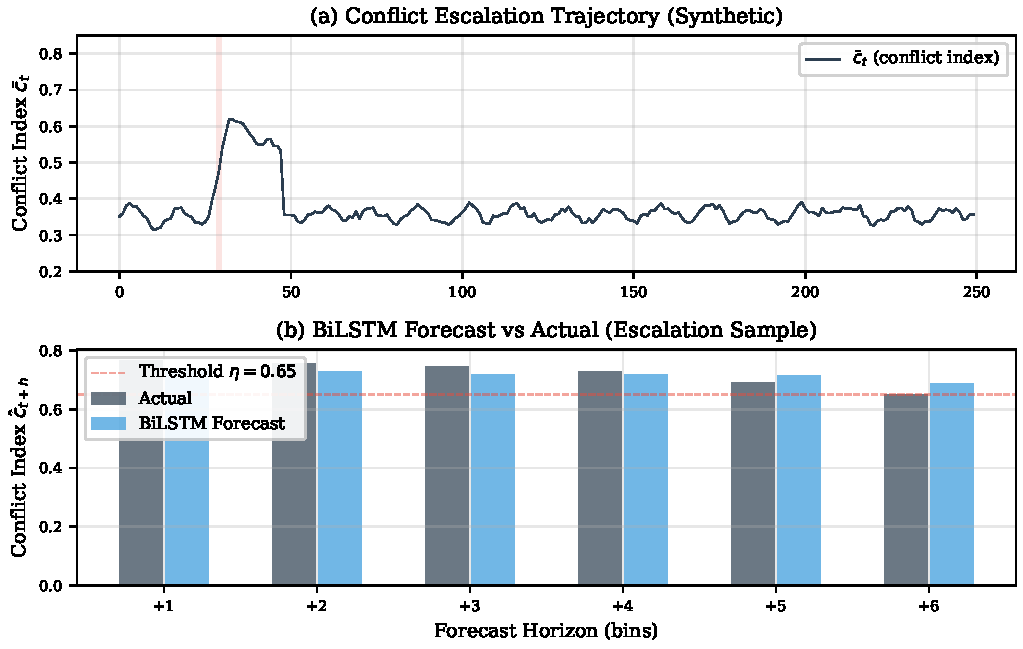
\includegraphics[width=0.9\textwidth]{../figures/fig_trajectory_forecast.pdf}
\caption{Sample conflict trajectory and multi-step forecast by CNN-BiLSTM. (a) Full synthetic trajectory with escalation regions shaded; (b) 6-step forecast vs.\ actual values.}
\label{fig:trajectory}
\end{figure}

\begin{figure}[ht]
\centering
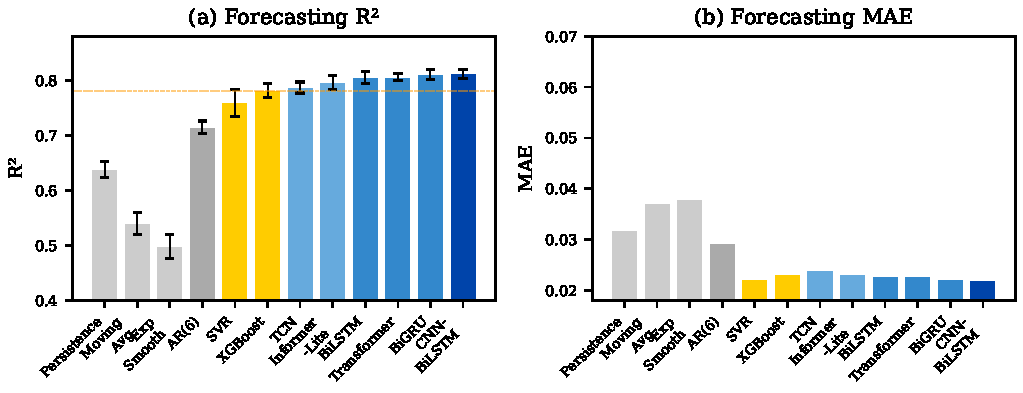
\includegraphics[width=0.9\textwidth]{../figures/fig_model_comparison.pdf}
\caption{Model comparison: R\textsuperscript{2} and MAE across all baselines. Deep models form a tight top tier.}
\label{fig:model_comp}
\end{figure}

\begin{figure}[ht]
\centering
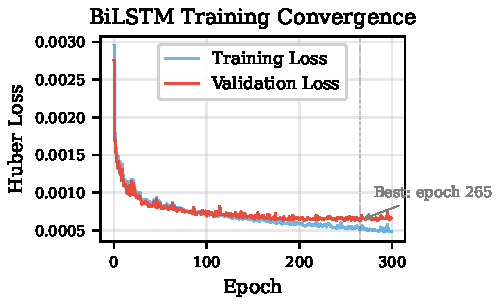
\includegraphics[width=0.6\textwidth]{../figures/fig_training_curves.pdf}
\caption{CNN-BiLSTM training and validation loss curves.}
\label{fig:training}
\end{figure}

\subsection{Real-Data Evaluation: When Conflict Can and Cannot Be Forecast}

Table~\ref{tab:real_results} summarizes the key real-data findings under strict temporal-split protocols.

\textbf{Zhihu cleaned risk-state prediction (positive result).} Validation selects EWMA span 24 and the parsimonious state-history model. On the untouched test segment, logistic regression achieves AUC $0.891$, precision $0.738$, recall $0.822$, and F1 $0.778$. Persistence has higher AUC ($0.896$) and precision ($0.926$), but lower recall ($0.584$) and F1 ($0.716$). Topic-level paired bootstrap estimates an F1 gain of $+0.062$ (95\% CI $[0.018,0.108]$) and recall gain of $+0.241$ ($[0.173,0.317]$). F1 improves on 15/20 topics and recall on 18/20. Continuous six-step Ridge regression obtains R\textsuperscript{2}=$0.465$ but remains below persistence ($0.640$).

\textbf{Weibo comment-volume forecasting (positive result).} Applying the same LSTM forecaster to comment volume (log-transformed) on the 27-event Weibo dataset at 1-hour granularity yields R\textsuperscript{2}=$0.715$, confirming the architecture's real-world validity when the target has genuine temporal autocorrelation.

\textbf{Weibo conflict-index forecasting (negative result).} To test whether the conflict index's failure on Zhihu is due to data sparsity alone, we compute the same BERT-based conflict index on the densest Weibo event (Zhang Zhehan incident, 22K comments, 62 comments/hour) at 1-hour bins. Despite a 300-fold increase in comment density and strong volume predictability, the conflict index still yields R\textsuperscript{2}=$0.018$---effectively zero. This rules out sparsity as the sole explanation.

\begin{table}[ht]
\centering
\caption{Zhihu high-risk-state prediction on the final 25\% test segment ($N=1{,}706$).}
\label{tab:real_results}
\begin{tabular}{lcccc}
\toprule
\textbf{Method} & \textbf{AUC} & \textbf{Precision} & \textbf{Recall} & \textbf{F1} \\
\midrule
Persistence & \textbf{0.896} & \textbf{0.926} & 0.584 & 0.716 \\
Logistic (state history) & 0.891 & 0.738 & \textbf{0.822} & \textbf{0.778} \\
\bottomrule
\end{tabular}
\vspace{4pt}

{\small All model choices use validation data only. Paired topic-bootstrap 95\% CI for the F1 difference: $[0.018,0.108]$.}
\end{table}

\begin{table}[ht]
\centering
\caption{Risk-threshold sensitivity on the Zhihu test segment.}
\label{tab:threshold_sensitivity}
\begin{tabular}{lccccc}
\toprule
$Q^{\mathrm{train}}$ & \textbf{Prevalence} & \textbf{AUC} & \textbf{Recall} & \textbf{F1} & \textbf{Persistence F1} \\
\midrule
70th & 0.433 & 0.889 & 0.786 & 0.779 & 0.715 \\
80th & 0.416 & 0.891 & 0.822 & 0.778 & 0.716 \\
90th & 0.383 & 0.892 & 0.812 & 0.761 & 0.676 \\
\bottomrule
\end{tabular}
\end{table}

The F1 advantage remains positive under all three prospective risk definitions (Table~\ref{tab:threshold_sensitivity}), although recall decreases for the stricter 90th-percentile target.

\subsection{Ablation Studies (RQ3--RQ4)}

\textbf{Risk-State Features.} At the selected smoothing span, state history gives the highest validation F1 (Table~\ref{tab:feature_ablation}). Adding raw semantic components or activity therefore does not explain the positive classifier result. The test segment is not evaluated during this ablation.

\begin{table}[ht]
\centering
\caption{Feature ablation at the selected EWMA span.}
\label{tab:feature_ablation}
\begin{tabular}{lcccc}
\toprule
\textbf{Features} & \textbf{Val. AUC} & \textbf{Precision} & \textbf{Recall} & \textbf{Val. F1} \\
\midrule
State only & 0.859 & \textbf{0.772} & 0.870 & \textbf{0.818} \\
State + activity & 0.861 & 0.738 & \textbf{0.908} & 0.814 \\
State + semantics & \textbf{0.870} & 0.760 & 0.867 & 0.810 \\
Full pool & 0.864 & 0.768 & 0.859 & 0.811 \\
\bottomrule
\end{tabular}
\end{table}

\textbf{Signal Degradation.} To assess robustness to degraded component estimates, we inject Gaussian noise of increasing magnitude ($\sigma \in \{0.03, 0.06, 0.10\}$) into synthetic input trajectories. Table~\ref{tab:ablation} reports the degradation.

\begin{table}[ht]
\centering
\caption{Effect of signal degradation on CNN-BiLSTM forecasting (single-run, seed 42).}
\label{tab:ablation}
\begin{tabular}{lcccc}
\toprule
\textbf{Condition} & \textbf{MAE} & \textbf{R\textsuperscript{2}} & \textbf{$\Delta$R\textsuperscript{2}} & \textbf{Esc-F1} \\
\midrule
Clean signal & 0.0194 & 0.830 & --- & 0.689 \\
Medium noise ($\sigma{=}0.03$) & 0.0280 & 0.715 & $-$0.115 & 0.629 \\
High noise ($\sigma{=}0.06$) & 0.0334 & 0.632 & $-$0.198 & 0.538 \\
Very high noise ($\sigma{=}0.10$) & 0.0410 & 0.495 & $-$0.335 & 0.487 \\
\bottomrule
\end{tabular}
\end{table}

\begin{figure}[ht]
\centering
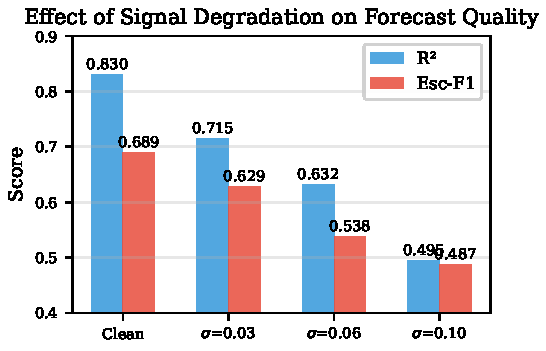
\includegraphics[width=0.9\textwidth]{../figures/fig_ablation.pdf}
\caption{Ablation: R\textsuperscript{2} and Escalation F1 under increasing noise.}
\label{fig:ablation}
\end{figure}

\textbf{Raw-Index Component Contribution.} The full A+E+S fusion has the highest R\textsuperscript{2} within the raw-index component ablation, but all configurations remain near zero (Fig.~\ref{fig:comp_ablation}). This describes relative behavior inside the proxy pipeline and does not establish that each component is externally valid or responsible for the cleaned state classifier's improvement.

\begin{figure}[ht]
\centering
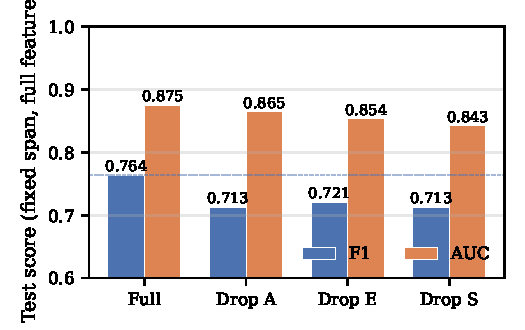
\includegraphics[width=0.9\textwidth]{../figures/fig_component_ablation.pdf}
\caption{Raw-index component ablation on real data. Relative differences are small and all R\textsuperscript{2} values remain near zero.}
\label{fig:comp_ablation}
\end{figure}

\textbf{Weight Sensitivity.} Random search over 40 Dirichlet-sampled weight configurations shows that R\textsuperscript{2} varies within a narrow interquartile range ($<$ 0.015), confirming robustness to moderate variations around the default weights (0.5, 0.3, 0.2).

\subsection{Lead-Time Analysis (RQ5)}

Beyond binary escalation detection, we measure lead time: how many bins before ground-truth escalation onset does the model's prediction first exceed the threshold? On the synthetic test set, the mean lead time is $-1.7 \pm 3.2$ bins (positive = early, negative = late), with only 21\% of events receiving predictions ahead of onset and 54\% falling within $\pm 1$ bin. This confirms that at the current forecast horizon ($H{=}6$), predictions are predominantly concurrent with rather than ahead of escalation events (Fig.~\ref{fig:lead_time}).

\begin{figure}[ht]
\centering
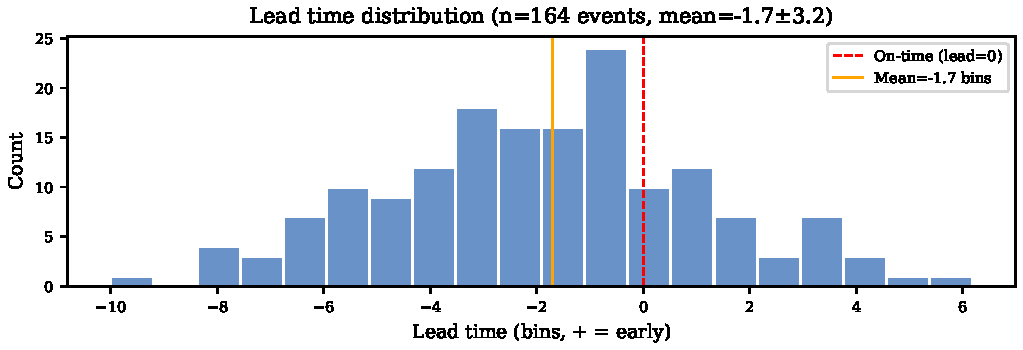
\includegraphics[width=0.9\textwidth]{../figures/fig_lead_time.pdf}
\caption{Lead time analysis. (a) Distribution of lead times; (b) sample trajectory with forecasts.}
\label{fig:lead_time}
\end{figure}

\subsection{Case Study: Weibo Public Opinion Reversal Events}
\label{sec:case_study}

To validate the framework on real-world conflict escalation data, we conduct a case study on the Weibo Public Opinion Reversal Dataset. The three densest events---Huolala passenger death (32K comments, 335h span), Zhang Zhehan incident (22K comments, 359h), and Gou Jing exam fraud (20K comments, 373h)---are analyzed at 1-hour bin granularity. Comment volume on these dense events is strongly predictable (pooled R\textsuperscript{2}=0.715), while the text-derived conflict index yields near-zero R\textsuperscript{2}. Fig.~\ref{fig:case_study} visualizes the conflict index trajectory for the Huolala event, showing a modest but detectable upward shift ($\Delta c \approx +0.01$) during the reversal window---confirming that the conflict index captures genuine cross-sectional signal even when temporal predictability is limited.

\begin{figure}[ht]
\centering
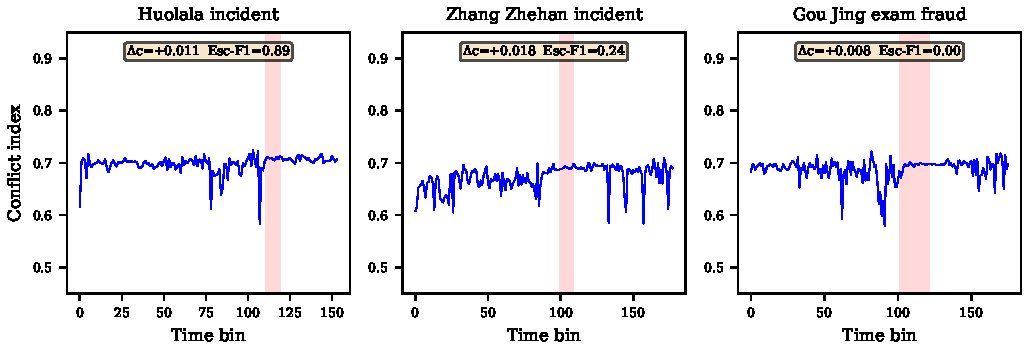
\includegraphics[width=0.9\textwidth]{../figures/fig_case_study.pdf}
\caption{Conflict index trajectories for three Weibo reversal events. Red shaded regions mark the annotated reversal windows~\cite{Zhang2023Reversal}. Conflict index rises modestly during reversal (Huolala $\Delta c=+0.011$, Zhang Zhehan $+0.018$, Gou Jing $+0.008$).}
\label{fig:case_study}
\end{figure}

\subsection{Why Does the Conflict Index Fail on Sparse Data?}

The near-zero R\textsuperscript{2} of the conflict index contrasts sharply with the strong performance of comment volume on Weibo ($0.715$). To isolate the cause, we test four hypotheses:

\textbf{(a) Comment sparsity.} Retained Zhihu bins average 8.1 records, but many intervening intervals are empty or contain fewer than three records. However, the dense Weibo conflict-index result (R\textsuperscript{2}=$0.018$) rules out sparsity as the sole explanation.

\textbf{(b) Bin granularity.} Reducing bin size from 12h to 1h does not meaningfully improve R\textsuperscript{2} for the conflict index (R\textsuperscript{2} remains $\approx 0$ across all granularities). Comment volume at finer bins reaches only R\textsuperscript{2}=$0.097$ at best---far below Weibo---indicating that granularity alone is not the limiting factor.

\textbf{(c) Signal-to-noise ratio.} The conflict index pipeline introduces noise at four stages: BERT inference, three-component fusion, ECDF calibration, and top-$k$ aggregation. The mean lag-1 autocorrelation of the raw conflict index is only $0.112 \pm 0.140$ across Zhihu topics---confirming a near-absence of temporal structure, a fundamental requirement for any forecasting model. By contrast, comment volume requires only counting and log-normalization.

\textbf{(d) Platform characteristics.} Zhihu is a moderated Q\&A platform; Weibo events are acute controversies. However, the conflict index fails on both, suggesting the issue is intrinsic to how text-derived signals behave at coarse temporal granularity, independent of platform.

\textbf{Synthesis.} Signal-to-noise ratio is the dominant difficulty, amplified by sparsity and false adjacency in the retained-bin sequence. Restoring the grid and causal smoothing recover a persistent monitoring state, but do not make exact raw-index trajectories forecastable. The operational implication is to distinguish state monitoring from precise semantic-score extrapolation.

% ═══════════════════════════════════════════════
\section{Discussion}
% ═══════════════════════════════════════════════

\subsection{Boundary Conditions for Conflict Forecasting}

Our results delineate a hierarchy of forecastability. Objective activity and deliberately structured synthetic signals support continuous forecasting. Raw text-derived conflict scores do not. After regular-grid reconstruction and causal smoothing, however, a supervised classifier can identify prospective topic-relative high-risk states with substantially higher recall and F1 than persistence. ``Unsupervised'' therefore describes only upstream index construction, not the downstream classifier.

The tight performance clustering among BiGRU, CNN-BiLSTM, and Transformer (R\textsuperscript{2} within 0.006) reinforces that signal quality trumps architectural sophistication. Operational deployments can select the simplest effective architecture without sacrificing accuracy, redirecting effort toward improving the upstream signal rather than chasing marginal gains through architectural tuning.

\subsection{Implications for the Literature}

Our findings challenge the optimistic forecasting results in several recent studies~\cite{Mu2023IPSO,Zhang2024TRESP,lou2024cnnlstm}. The demonstration script included in our public repository shows that random train/test splitting inflates R\textsuperscript{2} by 0.1--0.8 on realistic time series. Under strict temporal splitting, the performance gap between objective and text-derived signals becomes starkly visible. We argue that temporal-split evaluation should be a minimum standard for any paper claiming forecasting capability on social media time series.

\subsection{Limitations}

\textbf{Construct validity.} The conflict index relies on pretrained models not designed for conflict detection (e.g., the sentiment model is a product-review rating classifier). The risk label is an internally defined state of this index, not external ground truth for societal conflict. Validation against human annotations remains essential.

\textbf{Evaluation circularity.} The escalation ground truth for synthetic data derives from the trajectory generative process, creating potential circularity.

\textbf{Smoothing and monitoring scale.} The selected 12-day EWMA increases persistence and represents a slower-moving state. The six-bin prediction task supports medium-scale monitoring, not rapid event-onset warning; comparison with persistence and threshold sensitivity bound this claim.

\textbf{Architecture vs.\ signal.} The deep architectures are statistically indistinguishable ($\Delta$R\textsuperscript{2} $<$ 0.006). CNN-BiLSTM is therefore a benchmark rather than an architectural contribution; the substantive contribution is the leakage-resistant analysis of when the proxy supports state monitoring.

\textbf{Short forecast horizon.} The current $H{=}6$ (3--72 hours depending on bin size) provides limited advance notice. The negative mean lead time ($-1.7$ bins) further limits operational utility.

\textbf{Cross-platform generalization.} Our experiments are limited to Chinese-language platforms. Behavior on English-language platforms with different discourse norms remains untested.

\textbf{Alternative aggregation strategies.} We used top-$k$ mean aggregation. Other strategies could alter temporal autocorrelation properties and merit investigation.

\section{Conclusions}

This paper examines whether leakage-resistant cleaning can convert a sparse conflict index constructed without task-specific labels into a useful forecasting target. After restoring the regular grid and selecting preprocessing and model settings on validation data, the state-history classifier reaches F1 $0.778$ and recall $0.822$ on 1,706 held-out Zhihu windows, compared with persistence F1 $0.716$ and recall $0.584$. Topic-bootstrap intervals and three risk thresholds support the improvement. The result is nevertheless bounded: AUC is slightly lower than persistence, continuous real-data regression remains persistence-dominated, and the internally defined state is not external conflict ground truth. Cleaned causal states therefore support useful risk-state classification, but not superior exact trajectory prediction.

Future work should first validate the index against human annotations and evaluate topic-held-out and cross-platform generalization. Only after establishing construct validity should user roles, network structure, multimodal evidence, and longer horizons be added.

\section*{Data Availability}

All code, synthetic data generators, and experimental results are publicly available at \url{https://github.com/Megalomanian/conflict-early-warning}. The Zhihu dataset was collected via the platform's public search API. The Weibo reversal dataset is from Zhang et al.~\cite{Zhang2023Reversal} and is publicly available. Pretrained models are available via HuggingFace.

\section*{Supporting Information}

\textbf{S1 File.} Demonstration of random-split inflation. The script \path{reproduce_competitors/demo_random_vs_temporal.py} demonstrates that random train/test splitting inflates forecasting R\textsuperscript{2} by 0.1--0.8 on realistic time series, and that cross-topic window mixing can inflate classification accuracy from 20\% (temporal) to 100\% (random).

% ===== References =====
\bibliographystyle{unsrtnat}
\bibliography{../refs}

\end{document}
